\documentclass[12pt]{article}

\usepackage{natbib}
\usepackage{booktabs}
\usepackage{longtable}
\usepackage{xspace}
\usepackage{fullpage}
\usepackage{hyperref}
\usepackage{graphicx}
\usepackage{float}

\hypersetup{
colorlinks=true,       % false: boxed links; true: colored links
linkcolor=red,          % color of internal links (change box color with
%linkbordercolor)
citecolor=blue,       % color of links to bibliography
filecolor=magenta,   % color of file links
urlcolor=cyan           % color of external links
}

%% Global noindent
\setlength\parindent{0pt}

%% Comments
\newif\ifcomments\commentstrue

\ifcomments
\newcommand{\authornote}[3]{\textcolor{#1}{[#3 ---#2]}}
\newcommand{\todo}[1]{\textcolor{red}{[TODO: #1]}}
\else
\newcommand{\authornote}[3]{}
\newcommand{\todo}[1]{}
\fi

\newcommand{\wss}[1]{\authornote{blue}{SS}{#1}} %Spencer Smith
\newcommand{\jc}[1]{\authornote{red}{JC}{#1}} %Jacques Carette
\newcommand{\oo}[1]{\authornote{magenta}{OO}{#1}} %Olu Owojaiye
\newcommand{\pmi}[1]{\authornote{green}{PM}{#1}} %Peter Michalski
\newcommand{\ad}[1]{\authornote{cyan}{AD}{#1}} %Ao Dong

\usepackage{listings}
\usepackage{color}
\usepackage{xcolor}

\definecolor{dkgreen}{rgb}{0,0.6,0}
\definecolor{gray}{rgb}{0.5,0.5,0.5}
\definecolor{mauve}{rgb}{0.58,0,0.82}

%% Code blocks
\lstset{
  language=bash,
  aboveskip=3mm,
  belowskip=3mm,
  showstringspaces=false,
  columns=flexible,
  basicstyle={\small\ttfamily\color{white}},
  numbers=none,
  backgroundcolor = \color{black},
  commentstyle=\color{gray},
  stringstyle=\color{mauve},
  breaklines=true,
  breakatwhitespace=true,
  tabsize=3
}

\title{A Guide to Empirical Measures} 
\author{Ao Dong}
\date{\today}

\begin{document}

\maketitle

This document is a general guide to the implements of empirical measures.

There are several sections in this guide, with one tool to use in each of them,
and usually measures different aspect of a software package. There is no
mandatory order to use which tool first.

\section{git\_stats}
\subsection{Introduction}
Name: git\_stats

Source Code: \href{https://github.com/tomgi/git_stats}{GitHub repo}

\subsection{User Manual}
\label{git_stats_manual}
Official Manual: \href{https://github.com/tomgi/git_stats}{GitHub repo}

\subsection{Demo of Installation and Running the Tool}
This is the showcase of how to install and run this tool.

The installation steps on your machine may be different from this section.
Please refer to Section \ref{git_stats_manual}.

Hardware: a virtual machine with 8 cores and 16 GB RAM

OS: Debian GNU/Linux 9.11

\begin{enumerate}
\item Install ruby/gem environment
\begin{lstlisting}
apt-get install ruby ruby-nokogiri ruby-nokogiri-diff ruby-nokogumbo
\end{lstlisting}

Check the installation:
\begin{lstlisting}
gem --version
\end{lstlisting}
    
\item Install the tool
\begin{lstlisting}
sudo gem install git_stats
\end{lstlisting}
    
\item Prepare the target repo

Make sure the target repo (the repo to be analyzed, not the repo of this tool)
is on your machine.
In this demo, the target repo is downloaded from a GitHub repo:
\begin{lstlisting}
# change [git path] to the url of your target repo
git clone [git path]
# e.g. git clone https://github.com/nroduit/Weasis.git
\end{lstlisting}
    
\item Generate analytics
\begin{lstlisting}
# make sure [repo path] is the target repo path
# the [output path] can be anywhere you desire
git_stats generate -p [repo path] -o [output path]
# e.g. git_stats generate -p /home/user/git-stats/Weasis -o /home/user/git-stats/Weasis-analytics
\end{lstlisting}
    
\item View the analytics

View the analytic results by open [output path]/index.html with any browser or
other software supporting HTML web page format.
\begin{figure}[H]
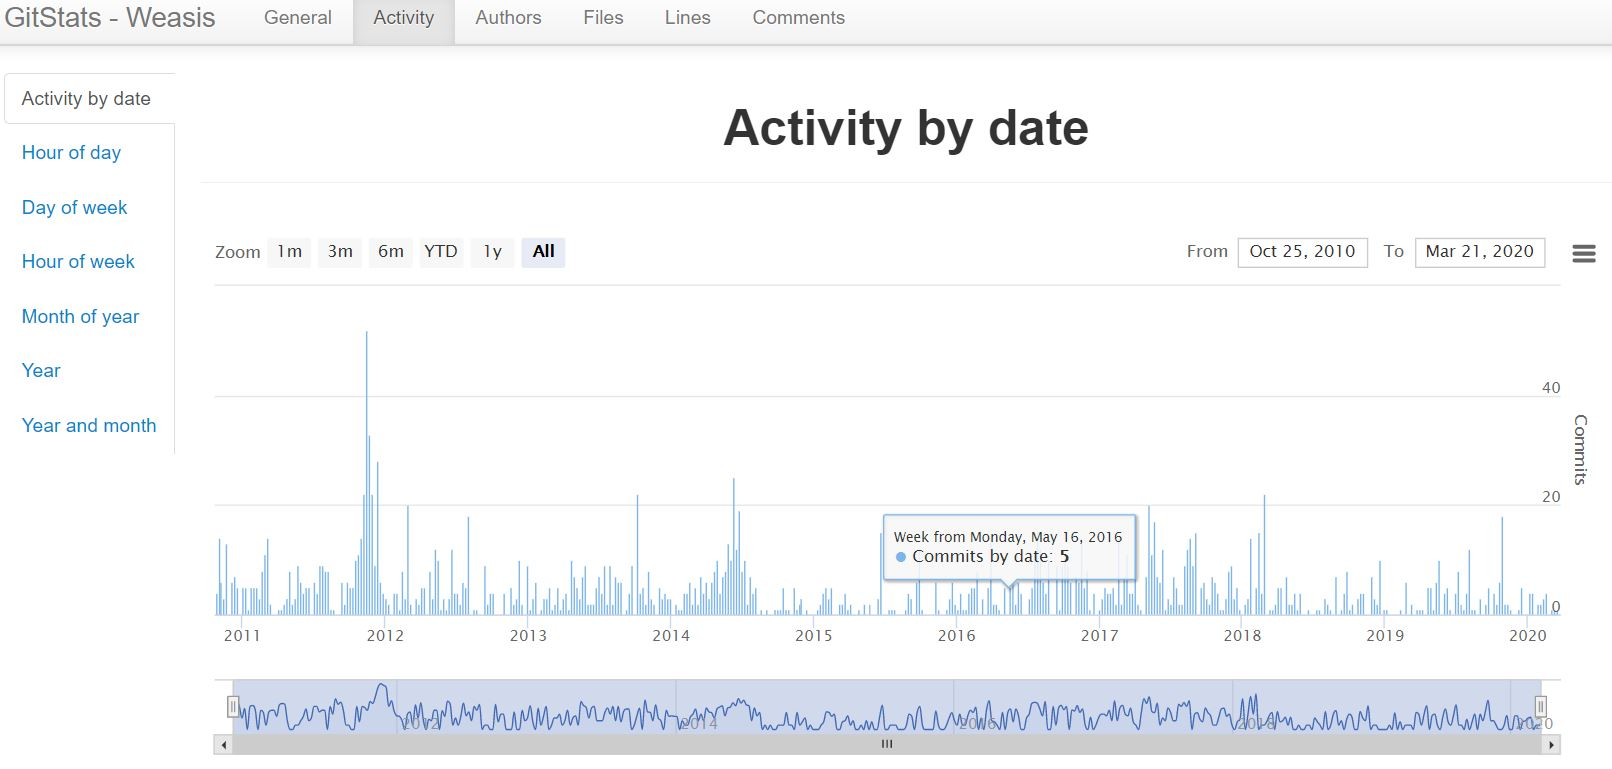
\includegraphics[scale=0.5]{git-stats-demo.JPG}
\end{figure}

\item Download the data

On most of the taps of this web page, the data can be downloaded for more
analytics by clicking the menu button beside the data-range section.
\end{enumerate}

\section{scc}
\subsection{Introduction}
Name: scc

Source Code: \href{https://github.com/boyter/scc}{GitHub repo}

\subsection{User Manual}
\label{scc_manual}
Official Manual: \href{https://github.com/boyter/scc}{GitHub repo}

\subsection{Demo of Installation and Running the Tool}
This is the showcase of how to install and run this tool.

The installation steps on your machine may be different from this section.
Please refer to Section \ref{scc_manual}.

Hardware: a virtual machine with 8 cores and 16 GB RAM

OS: Debian GNU/Linux 9.11

\begin{enumerate}
\item Install Golang

Follow the \href{https://golang.org/doc/install}{official instructions}, or the
following demo,

download the installation package:
\begin{lstlisting}
wget https://dl.google.com/go/go1.14.3.linux-amd64.tar.gz
\end{lstlisting}
    
unpack to /usr/local:
\begin{lstlisting}
sudo tar -C /usr/local -xzf go1.14.3.linux-amd64.tar.gz
\end{lstlisting}

use a text editor to open \textasciitilde/.profile, e.g.:
\begin{lstlisting}
nano ~/.profile
\end{lstlisting}

add the following lines to the end of this file:
\begin{lstlisting}
export GOPATH=$HOME/go
export PATH=$PATH:/usr/local/go/bin:$GOPATH/bin
\end{lstlisting}

save the file, and load the commands into the current shell instance:
\begin{lstlisting}
source ~/.profile
\end{lstlisting}

check the installation:
\begin{lstlisting}
go version
\end{lstlisting}

\item Install the tool
\begin{lstlisting}
go get -u github.com/boyter/scc/
\end{lstlisting}
    
\item Prepare the target repo

Make sure the target repo (the repo to be analyzed, not the repo of this tool)
is on your machine.
In this demo, the target repo is downloaded from a GitHub repo:
\begin{lstlisting}
# change [project path] to your desired folder
cd [project path]
git clone https://github.com/nroduit/Weasis.git
\end{lstlisting}

\item Generate analytics
\begin{lstlisting}
# make sure [repo path] is the target repo path
cd [repo path]
# use scc to generate analytics
scc
\end{lstlisting}
    
\item View the analytics

The results will be directly shown.
\begin{figure}[H]
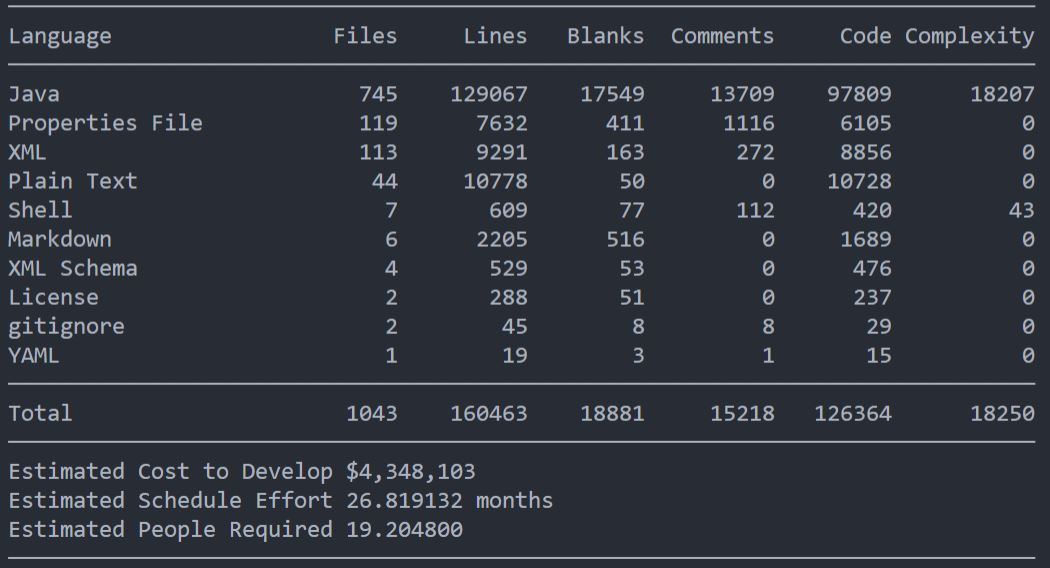
\includegraphics[scale=0.7]{scc-demo.JPG}
\end{figure}

\end{enumerate}

\end{document}